\documentclass[a4paper, 12pt,oneside]{memoir}
\usepackage[utf8]{inputenc}					% Sets encoding to UTF-8
\usepackage[T1]{fontenc}					% Expands font encoding
\usepackage[english]{babel}					% Sets language to english
\usepackage{amssymb}						% More mathematical symbols. Load before fonts
\usepackage{libertine, libertinust1math}
\usepackage{microtype}						% Dark typographic magic that makes the document more readable
\usepackage[hidelinks]{hyperref}
%\usepackage{geometry}

%% Linespacing
%\OnehalfSpacing
%\DoubleSpacing


\setlrmarginsandblock{3cm}{*}{1}
\setulmarginsandblock{3cm}{4cm}{*}


%% Page endings
%\flushbottom
%\raggedbottom
\sloppybottom


\checkandfixthelayout




%%%%%%%%%%%%%%%%%%%%%%%%%%%%%%%%%%
%%%%    FIGURES AND TABLES    %%%%
%%%%%%%%%%%%%%%%%%%%%%%%%%%%%%%%%%
\usepackage{graphicx}						% For inserting images
\usepackage{float}							% Greater control of figure placement
\usepackage[table]{xcolor}					% Colour different objects in the document
\usepackage{tikz}							% Draw figures with code
\usetikzlibrary{arrows, decorations.pathmorphing}
\usepackage{pdfpages}						% Insert pdfs into document


%% Folder with figures


%% Caption settings
\captionnamefont{\bfseries\footnotesize}
\captiontitlefont{\footnotesize}
\changecaptionwidth
\captionwidth{\marginparwidth}


%% For the front page
\newcommand{\projecttitle}{Threshold Pion Photoproduction off Nucleons using the Nuclear Model with Explicit Pions}
\newcommand{\projectauthor}{Martin Mikkelsen }
\newcommand{\projectauthorID}{201706771}
\newcommand{\projectsupervisor}{Dmitri Fedorov}
%\newcommand{\projectcosupervisor}{Georg M. Bruun}
\newcommand{\projectdate}{November 2022}
\newcommand{\projectdepartment}{Department of Physics and Astronomy}
\newcommand{\projectuniversity}{Aarhus University}
%\newcommand{\projectfrontpagefigure}{File Name of Figure}		% Comment out if no figure is wanted.
\begin{document}
\pagestyle{empty}
\begin{center}
	
	\fontsize{26pt}{29pt}\selectfont
	
	\textsc{\projecttitle} \par
	
	\vspace{0.75cm}
	
	\fontsize{20pt}{24pt}\selectfont
	
	\projectauthor -- 
	\projectauthorID \par
	\vspace{0.5cm}
	
	\fontsize{16pt}{16pt}\selectfont
	Master's Thesis
	
	\vspace{0.2cm}
	\begin{center}
	\begin{figure}[H]
		\centering
		\hspace*{0cm}
		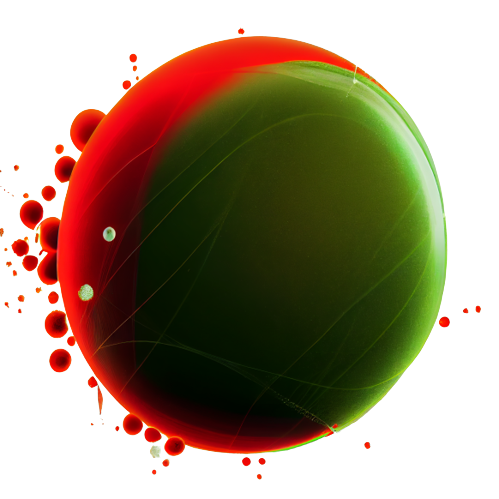
\includegraphics[width=0.55\linewidth]{Pion-NucleonSystem.png}
		\label{fig:pion-nucleonsystem}
	\end{figure}
\end{center}
	\vspace{0.2cm}
	
	\fontsize{20pt}{24pt}\selectfont
	 Supervisor: \projectsupervisor \par
	
	\vspace{1cm}
	
	\fontsize{18pt}{22pt}\selectfont
	
	\textsc{\projectdepartment} \par
	\textsc{\projectuniversity} \par
	
	\vspace{1cm}
	
	\projectdate
\end{center}
\vfill
\noindent

\includegraphics{Logo_Department_en}
\hfill

\includegraphics{segla1b}
\end{document}